\documentclass[conference]{IEEEtran}
\IEEEoverridecommandlockouts

\usepackage{amsmath,amssymb,amsfonts}
\usepackage{textcomp}
\usepackage{graphicx}
\usepackage{xcolor}
\usepackage{array}
\usepackage{booktabs}
\usepackage{siunitx}
\usepackage[backend=bibtex,
            language=english,
            autolang=other,
            style=ieee]{biblatex}
\addbibresource{bib.bib}
\usepackage[hidelinks]{hyperref}
\usepackage[capitalize]{cleveref}
\usepackage[nonumberlist]{glossaries}
\makenoidxglossaries
\loadglsentries{abbr}
\usepackage[font=small]{caption}
\usepackage{subcaption}
\AtBeginBibliography{\footnotesize}
\newcommand{\dataset}{\textsc{DATASET}}

\def\BibTeX{{\rm B\kern-.05em{\sc i\kern-.025em b}\kern-.08em
    T\kern-.1667em\lower.7ex\hbox{E}\kern-.125emX}}

\input{auto_names}

\usepackage{orcidlink}

\defineauthors[false]{gilles, jarne, daan, bert, gustav}

\usepackage{array}
\newcolumntype{H}{>{\setbox0=\hbox\bgroup}c<{\egroup}@{}}

\usepackage{fontawesome}
    
\begin{document}

\title{ARFT: A Synchronized Multimodal RF-Acoustic Dataset for Positioning in Distributed Environments}

%ARFT (Acoustic-Radio Fusion at Techtile)

\author{
%%%% AUTHORS %%%%
\IEEEauthorblockN{%
Daan Delabie\,\orcidlink{0000-0002-0089-3633}\IEEEauthorrefmark{1},
Jarne Van Mulders\,\orcidlink{0000-0003-4103-3290}\IEEEauthorrefmark{1},
Bert Pyck\,\IEEEauthorrefmark{1},
Gustav Nilsson Gisleskog\,\orcidlink{0009-0006-3230-8319}\IEEEauthorrefmark{2},
Gilles Callebaut\,\orcidlink{0000-0003-2413-986X}\IEEEauthorrefmark{1},
}
%%%% AFFILIATIONS %%%%% ...
\IEEEauthorblockA{\IEEEauthorrefmark{1}% 2nd affiliations
KU Leuven, Department of Electrical Engineering, KU Leuven Ghent, Belgium}
\IEEEauthorblockA{\IEEEauthorrefmark{2}% 2nd affiliations
Lund Univerisity, Centre for Mathematical Sciences, Lund, Sweden} %\\
}

\maketitle

\begin{abstract}
This paper documents the \gls{arft} dataset, a synchronized measurement campaign for distributed wireless sensing and positioning in the Techtile testbed. Ultrasonic and \gls{rf} signals are simultaneously transmitted and captured at multiple positions in a 2D spatial grid inside the Techtile testbed.
Each acquisition cycle corresponds to one rover stop, one position sample, one acoustic recording and one \gls{rf} snapshot. The \gls{rf} modality is recorded as per-host pilot measurements and released as \gls{csi} tensors for 42 antennas mounted at the ceiling of the room. The acoustic chirp is recorded with 91 synchronized microphones and transmitted by a synchronized quasi omni-directional speaker. The campaign spans 5011 spatial position samples spanning  a 5.57~m by 2.89~m area with complete RF and acoustic data. We detail how the measurements are recorded, quantify per-experiment coverage, describe the RF and acoustic data contents, and explain how the aligned modalities support RF-only, acoustic-only, and joint positioning workflows. Furthermore, a static acoustic positioning pipeline that performs anchor selection, pulse-compression ranging, and \gls{ls} localization is elaborated. 
\end{abstract}

\begin{IEEEkeywords}
dataset, localization, RF, acoustics, multimodal sensing
\end{IEEEkeywords}

% \tableofcontents

\section{Introduction}
\glsresetall

Large-scale experimental datasets have become increasingly important for wireless communication, sensing, and positioning research because they decouple algorithm development from scarce hardware testbed time and expose downstream users to realistic synchronization errors, coverage gaps, and multimodal alignment constraints. Recent multimodal releases such as DeepSense~6G show how carefully documented measurement assets can accelerate communication-aware sensing research well beyond their original experimental purpose~\cite{alkhateeb2023deepsense}. In parallel, Techtile was designed exactly as the kind of room-scale, distributed, synchronized infrastructure needed to create such assets for beyond-5G and 6G experimentation~\cite{techtilePrimer,techtileOpen6g}.

\dataset{} packages one concrete synchronized measurement campaign on top of Techtile. It includes the acquisition stack, rover control, acoustic tooling, \gls{rf} measurement scripts, parsing code, completeness checks, processed data products, and notebook-based analysis workflow used during the campaign. This makes the release more than a collection of files: it is the operational record of how synchronized rover, acoustic, and \gls{rf} measurements were acquired and transformed into analysis-ready products.

The closest dataset families motivate, but do not duplicate, this measurement design. DeepSense~6G provides a broad multi-scenario resource for communication-aware multimodal sensing, with RF measurements aligned to exteroceptive sensing modalities such as camera, radar, LiDAR, and position information~\cite{alkhateeb2023deepsense}. Its scale and scenario diversity are complementary to the present release. \dataset{} instead targets an indoor distributed positioning setting in which each acquisition cycle joins a ceiling-aperture \gls{rf} snapshot, an ultrasonic room response, and a motion-capture ground-truth pose at the same rover stop.

Indoor \gls{csi} localization work has established the utility of fingerprinting and learning-based position inference from channel measurements~\cite{kazemi2022csifingerprint,kordi2024survey,dai2023wifi}. Massive-MIMO and distributed-MIMO studies further show that large or spatially distributed RF apertures can provide richer spatial structure for fine-grained localization and data-driven channel modeling~\cite{li2022massivemimo,euchner2022bigcsidata}. These resources are essential for RF-only positioning research, but they generally do not provide synchronized acoustic waveforms recorded at the same physical pose. Conversely, acoustic positioning datasets and Techtile acoustic studies emphasize time-of-arrival, room impulse response, and microphone-array processing in the audible or ultrasonic domain~\cite{techtileAcoustic2022}. They typically do not include phase-coherent distributed RF channel observations that can be fused cycle by cycle with the acoustic traces.

This places \dataset{} between three established lines of work: multimodal sensing datasets, RF \gls{csi} localization datasets, and acoustic positioning datasets. Its distinguishing element is not merely that several files are released, but that the same orchestrator cycle defines the rover pose, acoustic capture, and distributed \gls{rf} measurement. The cycle-level key makes the RF and acoustic products directly joinable, while Techtile's shared synchronization and calibration infrastructure makes the distributed RF observations phase-coherent across the active ceiling aperture~\cite{syncWptTechtile}. The release also follows open-science dataset practice by exposing processing scripts, completeness checks, NetCDF products, and notebooks rather than only final figures or summary metrics~\cite{dss6g}.

Relative to earlier Techtile infrastructure and acoustic-only work, \dataset{} contributes a dense scanned campaign with a co-located RF-acoustic rover payload rather than only platform characterization or acoustic measurements. Relative to DeepSense~6G, the distinguishing modality pairing is synchronized \gls{rf}+acoustic propagation inside a controlled indoor distributed aperture rather than broad outdoor RF-perception sensing. Relative to pure \gls{csi} datasets, the distinguishing capability is cycle-level synchronization of phase-coherent distributed \gls{rf} measurements with raw acoustic waveforms, common ground truth, and an open processing workflow.

This paper is intentionally not framed as a benchmark paper for a specific estimator, classifier, or neural architecture. Its purpose is narrower and more practical: to document the experiments that were actually run, quantify what is currently complete in the released data products, and explain what \dataset{} already enables a researcher to do. In that sense, the paper serves as a rigorous companion to the data release. It reconstructs the measurement workflow, summarizes the campaign experiment by experiment, clarifies how the NetCDF products should be interpreted, and distinguishes between the total logged campaign and the presently usable tri-modal subset.

Three aspects of \dataset{} are especially worth documenting. First, the acquisition is genuinely synchronized at the level of the physical rover stop: one orchestrator cycle corresponds to one commanded rover position, one Qualisys sample, one acoustic capture, and one \gls{rf} cycle. Second, the processed products are already structured for downstream use, with explicit availability masks and notebook-backed analysis examples. Third, completeness is uneven across experiments, which makes it essential to state clearly what parts of the campaign support \gls{rf}-only analysis and what parts support fully aligned \gls{rf}+acoustic+position analysis.

The remainder of the paper is as follows. \Cref{sec:platform} describes the platform and acquisition workflow. \Cref{sec:campaign} quantifies the campaign and its present coverage. \Cref{sec:capabilities} discusses the recorded data products and the positioning capabilities already exposed in the analysis workflow. \Cref{sec:discussion} concludes with the main interpretation caveats and current limitations.

\section{Platform and Acquisition Workflow}
\label{sec:platform}

\begin{figure*}[t]
    \centering
    % \begin{subfigure}[b]{0.48\textwidth}
    %     \centering
    %     \includegraphics[width=\linewidth]{figures/techtile-room-overview.jpg}
    %     \caption{Wide view of the Techtile measurement room used for the campaign.}
    % \end{subfigure}
    % \hfill
    \begin{subfigure}[t]{0.48\textwidth}
        \centering
        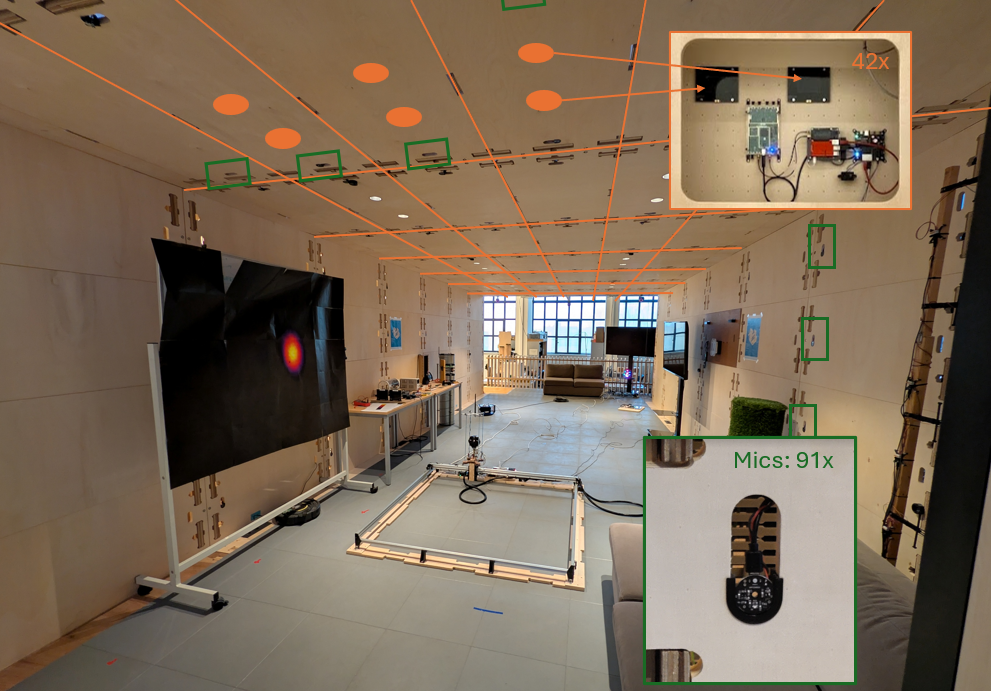
\includegraphics[height=5cm]{figures/techtile-room-setup.png}
        \caption{Measurement setup showing the rover frame and room instrumentation.}
    \end{subfigure}\hspace{2cm}%
    \begin{subfigure}[t]{0.32\textwidth}
        \centering
        \includegraphics[height=5cm]{figures/holder.jpg}
        \caption{Close-up of the rover-mounted payload combining the \gls{rf} antenna and the omnidirectional acoustic speaker on a common holder.}\label{fig:rover}
    \end{subfigure}
    \caption{Visual overview of the ARFT measurement setup, from room-scale deployment to the co-located RF-acoustic payload on the rover. \vspace{-3mm}}
    \label{fig:measurement-setup-photos}
\end{figure*}

ARFT is collected inside Techtile, a room-scale distributed testbed intended for communication, sensing, positioning, and related 6G experiments~\cite{techtilePrimer,techtileOpen6g, techtile-acoustic}. Techtile is built around 140 detachable tiles with Ethernet-based power, communication, and synchronization. It featurs a Qualisys-based sub-centimeter tracking system, 2D sampling robot, and 42 phase-coherent antennas operating at 920~MHz~\cite{syncWptTechtile,geomWpt2026,dliSuppression2026}. The transmit antenna is not phase-coherent with the receiving antennas.\footnote{This implies that the phase information should be interpreted relative to the other recived phases and should not be considered absolute. For instance, to determine the path length using the phase rotation between the transmitter and receiver.} For the campaign documented in this paper, the measurement rig (\cref{fig:rover}) combines an ultrasonic speaker and an \gls{rf} \gls{ue} antenna on a common mechanical mount so that the acoustic and \gls{rf} channels are sampled at the same physical 2D rover location. Ground-truth position is provided by the Qualisys system. The physical measurement environment is illustrated in \cref{fig:measurement-setup-photos}.



\subsection{Positioning and Measurement Procedure}

The measurements are coordinated by a central orchestrator, that coordinates the movement of the rover, position acquisition and RF and acoustic sampling.

\subsubsection{Orchestator}
The acquisition stack is organized around two control layers. The deployment layer pushes code and settings to the clients and starts the long-lived services. The orchestration layer then coordinates one end-to-end measurement cycle across rover motion, position logging, acoustics, and \gls{rf} synchronization. 
First, the rover moves to the commanded waypoint. Then the system records one fresh ground-truth Qualisys position sample at that stop. Afterward, the acoustic client records one chirp-response capture. Finally, the \gls{rf} orchestrator triggers one synchronized \gls{rf} cycle across the participating radio elements.

\subsubsection{Rover}
Both an antenna and speaker are mounted on a rover xy-plotter, as depicted in \cref{fig:rover}. The rover follows a reproducible multi-resolution scan over an $1.23 \times 1.23$~m work area. It performs a sweep over the area and with each iterations the density increases. Hence, the density of the collected samples is related to the total measurement time per area. This can be observed in \cref{fig:samples}. In particular, the rover planner uses a square spiral seven-sweep multi-resolution scan whose spacing is progressively reduced from 120 mm to approximately 50 mm. This makes the measurement process dense enough for spatial visualization while remaining operationally tractable for a multi-modal campaign.

\begin{figure}[t]
    \centering
    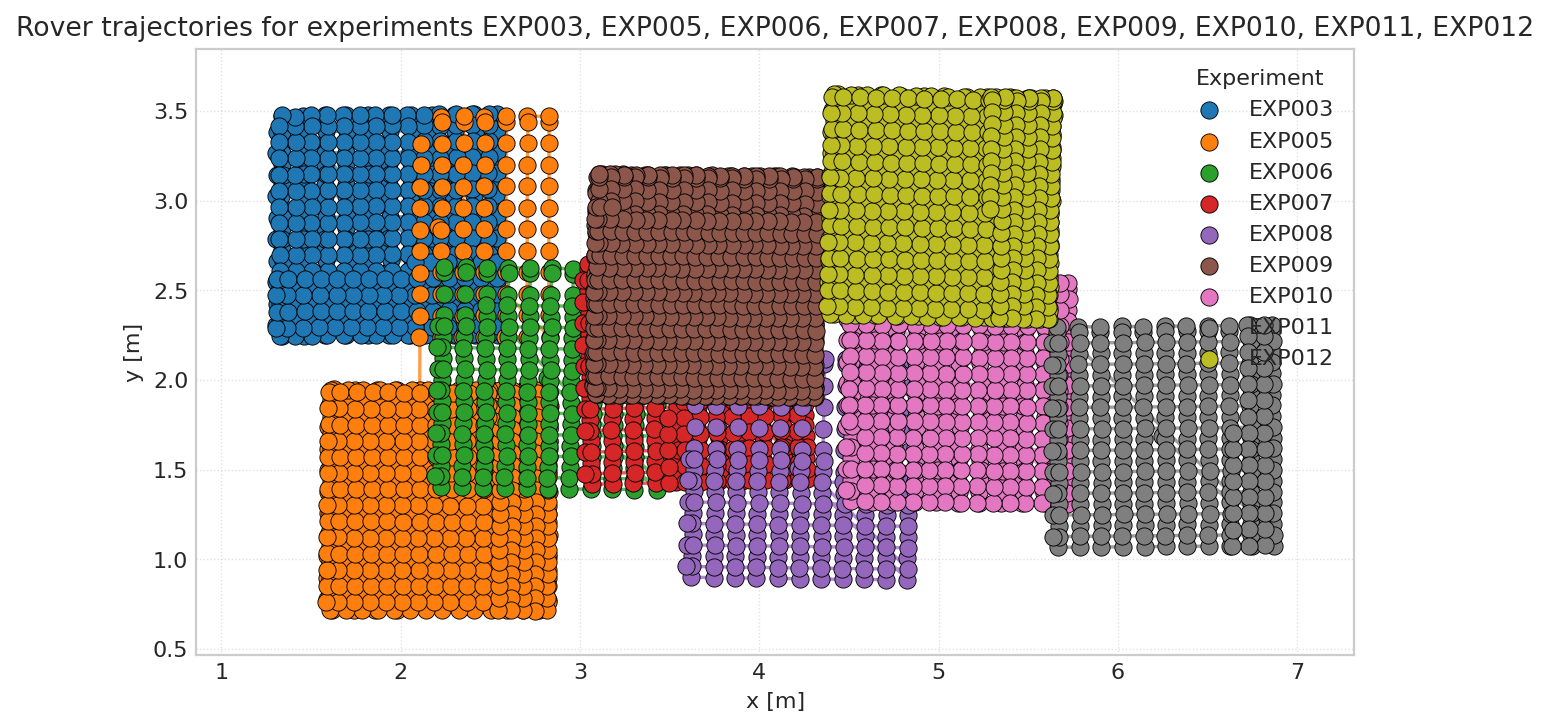
\includegraphics[width=\linewidth]{figures/notebook-exports/measurement_locations_trajectory.png}
    \caption{Trajectory and sampled measurement locations. \vspace{-3mm}}\label{fig:samples}
\end{figure}

\subsubsection{Positioning Ground Truth}
Ground-truth positioning is provided by the Qualisys system. 6 Miqus M3 cameras are installed, resulting in a 3D standard deviation on the accuracy of 1.25 mm.  After every completed rover move, the orchestrator requests one fresh $(x,y,z)$ position update. Note that in this dataset, the rover only moves in the $(x,y)$ plane, but the $z$-coordinates are stored as well. The reported $z$-coordinate is positioned at the bottom of the transmitter antenna.

\subsection{RF Orchestrator and Measurements}

The active \gls{rf} aperture used by the reciprocity workflow is the Techtile ceiling group: 42 receiver tiles\footnote{
Column \texttt{A} until \texttt{G} and row 5 until 10, covering \texttt{A05} until \texttt{G10}}. The campaign configuration uses the \gls{rf} measurements at 920~MHz with a 250~kS/s sample rate and receiver gain of 80.  

At each rover stop, the \gls{rf} orchestrator waits for an \texttt{ALIVE}  from all the tiles, publishes a  \texttt{SYNC} message, and waits for the corresponding \texttt{DONE} quorum before reporting completion to the main orchestrator. Techtile is further synchronized via a pulse-per-second distribution for time alignment, a shared 10~MHz reference for frequency alignment, and reciprocity-based calibration for front-end phase alignment~\cite{syncWptTechtile}. 

Each receiver stores one pilot-response record per cycle containing the measured pilot phase and amplitude. The reciprocity client estimates a circular-mean pilot phase from the captured IQ samples and pairs it with an \gls{rms} pilot amplitude, post-processing then applies cable-phase correction and converts the result into one complex \gls{csi} value per ceiling antenna. A single physical stop therefore produces a vector of up to 42 phase-coherent complex \gls{csi} observations across the active ceiling receivers. Currently, the dataset is limited to single-band \gls{csi} only.

\subsection{Acoustic Measurements}
The acoustic modality uses the rover-mounted ultrasonic speaker as the active source and the 91 distributed room microphones as fixed receivers. An opposite acoustic dataset in the same environment with the speakers being the anchors and a microphone being the mobile node was used and presented in~\cite{Echoes_of_accuracy, dataset_ultrasound_techtile}. Here, the speaker combines multiple Kemo L010 speakers in a dodecahedron shape forming a quasi-omni-directional ultrasonic speaker. The custom build microphone modules consist of IMP23ABSU \gls{mems} microphones combined with a pure analogue amplifier. One acoustic capture emits a 30~ms linear chirp from 20 to 40~kHz at a 250~kS/s sample rate. The acquisition task records a window twice as long as the excitation so that the direct arrival and the multipath components are preserved in the received signal to make the dataset more usable. The acoustic parameters of the Techtile environment were reported in~\cite{techtile-acoustic}. Techtile is a challenging environment in acoustic terms, with high reverberation and external noise factors. Due to the reverberation time ($\text{RT}_{60}$) of 0.4 s, an acoustic measurement can only take place with this low update rate to exclude interference across measurements. Therefore the acoustic data should be handled as a static dataset. In the current release configuration, these received chirp signals are stored directly rather than being reduced to only deconvolved impulse responses.

On the hardware side, the acoustic hardware shares the same \gls{daq} and thus reference clock, ensuring nanosecond synchronization between output and input tasks. A hardware start triggering ensures that the speaker emission and microphone sampling are aligned within one capture. Each saved acoustic data capture stores the chirp settings together with a microphone label, microphone coordinates, and the recorded waveform samples. The acoustic parser later reorganizes these runtime files into per-experiment waveform tensors indexed by experiment, cycle, microphone label, and sample index. Because the acoustic source and the \gls{rf} antenna are co-located on the rover, the acoustic traces and \gls{rf} snapshots refer to the same physical rover pose, except for a $z$-dimension offset as depicted in Fig.~\ref{fig:measurement-setup-photos} 

\begin{table}[t]
    \centering
    \caption{Key acquisition settings reconstructed from the campaign configuration.}
    \label{tab:config}
    \setlength{\tabcolsep}{4pt}
    \begin{tabular}{p{0.42\columnwidth}p{0.5\columnwidth}}
        \toprule
        Parameter & Value \\
        \midrule
        Testbed & Techtile distributed room-scale infrastructure \\
        Active \gls{rf} aperture & 42 ceiling receiver tiles (\texttt{A05}--\texttt{G10}) \\
        \gls{rf} excitation & Continious waveform pilot \\
        Center frequency & 920 MHz \\
        RF sample rate & 250 kS/s \\
        Receiver gain & 80 \\
        Positioning system & Qualisys \\
        Acoustic rig & ultrasonic speaker co-mounted with the \gls{rf} antenna, 91 microphones in walls and ceiling \\
        Acoustic excitation & 20--40 kHz linear chirp, 30 ms at 250 kS/s \\
        Runtime recording & rover CSV logs with pose, per-host \gls{rf} pilot logs, per-cycle acoustic waveform captures \\
        Rover sweep plan & 7 sweeps with nominal spacings 120, 120, 90, 90, 67.5, 67.5, and 50.6 mm\\
        \gls{rf} sync group & 43 synchronized subscribers in the pilot-synchronization loop \\
        Cycle semantics & 1 rover stop + 1 position sample + 1 acoustic capture + 1 \gls{rf} cycle \\
        \bottomrule
    \end{tabular}
\end{table}

\Cref{tab:config} highlights the key acquisition setting that were used to collect the ARFT dataset. Post-processing begins after acquisition. The \gls{rf} parser scans the per-host result files, extracts complex pilot measurements, applies cable correction, joins the result with rover positions, filters consecutive duplicate positions using a tolerance derived from the rover configuration, and writes one merged NetCDF. The acoustic parser produces a separate per-experiment NetCDF of recorded waveforms. ARFT therefore preserves both the runtime logs and the processed analysis data. The latter ultimately forms the merged dataset.

\section{Experimental Campaign and Coverage}
\label{sec:campaign}

\begin{table*}[t]
    \centering
    \caption{Per-experiment campaign summary detailing the number of collected samples per type. 
    % Coordinate ranges are in meters.
    }
    \label{tab:experiments}
    \scriptsize
    \setlength{\tabcolsep}{5pt}
    \begin{tabular}{lccccccc}
        \toprule
        Experiment & $x$ range & $y$ range & Rover cycles & \gls{rf} cycles & Acoustic cycles & Tri-modal cycles \\
        \midrule
        % EXP001 & [1.15, 1.75] & [2.55, 3.16] & 791  & 0    & 0    & 0 \\
        % EXP002 & [0.81, 2.05] & [2.26, 3.50] & 914  & 0    & 0    & 0 \\
        EXP003 & [1.31, 2.54] & [2.25, 3.48] & 529  & 529  & 529  & 529 \\
        % EXP004 & [1.92, 2.54] & [2.25, 3.48] & 19   & 0    & 0    & 0 \\
        EXP005 & [1.58, 2.83] & [0.71, 3.47] & 777 & 777  & 1618 & 777 \\
        EXP006 & [2.19, 3.44] & [1.39, 2.63] & 238  & 238  & 238  & 238 \\
        EXP007 & [3.01, 4.27] & [1.42, 2.68] & 378  & 378  & 379  & 378 \\
        EXP008 & [3.59, 4.84] & [0.89, 2.13] & 201  & 201  & 201  & 201 \\
        EXP009 & [3.07, 4.32] & [1.90, 3.15] & 1355 & 1355 & 1356 & 1355 \\
        EXP010 & [4.48, 5.73] & [1.31, 2.55] & 458  & 458  & 458  & 458 \\
        EXP011 & [5.63, 6.87] & [1.07, 2.31] & 291  & 291  & 291  & 291 \\
        EXP012 & [4.38, 5.64] & [2.34, 3.60] & 784  & 784  & 785  & 784 \\
        \bottomrule
    \end{tabular}
\end{table*}

The ARFT dataset campaign contains 12 named experiments (\texttt{EXP001}--\texttt{EXP012}). Across those runs, the recorded rover coordinates span approximately 0.81~m to 6.87~m in the Qualisys $x$-axis and 0.71~m to 3.60~m in the $y$-axis. The experiments are not all mapped to the same spatial subregion, which is evident from the per-experiment coordinate ranges in \cref{tab:experiments} and \cref{fig:samples}. The ARFT dataset contains 5011 tri-modal spatial samples. As can be observed, not all experiment runs, constitute the same number of samples and density.
% This corrected tri-modal subset spans 5.57~m in the $x$ direction and 2.89~m in the $y$ direction, corresponding to a 16.09~m$^2$ axis-aligned bounding box.

% Several observations follow directly from \cref{tab:experiments}. First, the campaign is not uniformly complete. EXP003, EXP006, EXP008, EXP010, and EXP011 are fully aligned. EXP007, EXP009 and EXP012 are nearly complete, each missing only one \gls{rf} and rover cycle. EXP005 contributes a large acoustic subset, but lacks \gls{rf} and rover cycles. Finally, EXP001, EXP002, and EXP004 provide rover coverage but not processed \gls{rf} or acoustic cycles in the present release.

% The campaign should therefore be interpreted as a layered asset rather than a single homogeneous benchmark. If the research question is purely acoustic-spatial, the usable set is materially larger than if joint \gls{rf}+acoustic analysis is required.

\section{Recorded Data Products and Positioning Capabilities}
\label{sec:capabilities}

ARFT exposes several distinct data products, each corresponding to a different layer of the workflow. At acquisition time, the rover logger writes one CSV row per completed move, the \gls{rf} clients write one runtime record per hostname and cycle, and the \gls{rf} orchestrator writes one YAML summary entry per synchronized cycle. The post-processing path then converts these operational files into analysis-ready NetCDF products. The use of hierarchical NetCDF products for the released tensors is also consistent with broader 6G testbed efforts that standardize reusable measurement datasets on top of NetCDF/HDF5 storage backends~\cite{dss6g}.

The current merged \gls{rf} NetCDF aggregates EXP003 and EXP005--EXP012 and has dimensions \texttt{experiment\_id} $\times$ \texttt{cycle\_id} $\times$ \texttt{hostname}. Its main variables are \texttt{csi\_real}, \texttt{csi\_imag}, \texttt{csi\_available}, \texttt{rover\_x}, \texttt{rover\_y}, \texttt{rover\_z}, and \texttt{position\_available}. One physical \gls{rf} observation is reconstructed as \texttt{csi\_real} $+ j\,\texttt{csi\_imag}$, while \texttt{csi\_available} indicates whether a given \texttt{(experiment\_id, cycle\_id, hostname)} tuple is populated. This design gives the user both direct array access and an explicit validity mask.

The \gls{rf} product should be interpreted as a distributed spatial fingerprint of the rover location. Each cycle yields a 42-element complex vector over the ceiling tiles, derived from the per-host pilot phase and amplitude measurements after cable correction. Across the 5011 populated \gls{rf} cycles in the merged file, the dataset stores 210068 tile-level complex \gls{csi} samples. Host coverage is also strong: 4617 of the 5011 \gls{rf} cycles contain all 42 ceiling-tile entries, and the remaining 394 cycles contain 41 entries. In other words, the typical measurement point is not a sparse partial vector but a nearly complete 42-element spatial snapshot. This makes the \gls{rf} modality directly usable for fingerprint-based positioning, for geometry-aware inference that exploits the distributed aperture, and for learning spatial channel maps that are later inverted for localization.

The acoustic product complements this with waveform-level information. The acoustic pipeline writes one NetCDF per experiment with waveform data organized on \texttt{(experiment\_id, cycle\_id, microphone\_label, sample\_index)}. Each stored trace corresponds to the chirp response recorded by a microphone at the same rover stop as the paired \gls{rf} snapshot. The acoustic modality therefore preserves time-domain propagation structure such as direct-path timing, reverberation, and multipath signatures. These traces can be used for acoustic fingerprinting, feature extraction for position regression or classification, or model-based processing that uses arrival-time and room-response cues for localization.

The key capability is tri-modal alignment. Because the acoustic and \gls{rf} parsers use the same \texttt{(experiment\_id, cycle\_id)} key, ARFT supports direct cycle-level joining between rover position, tile-level \gls{rf} channel measurements, and raw microphone waveforms. Since each cycle also has a ground-truth rover pose from Qualisys, the release supports three natural positioning regimes: RF-only positioning, acoustic-only positioning, and joint multimodal positioning in which both feature sets are fused against the same $(x,y,z)$ target. \Cref{fig:rf-acoustic-position-waveforms,fig:csi-position-heatmaps} show two notebook-derived views of this alignment and \gls{rf} structure: one cycle-level acoustic waveform matrix joined to a selected \gls{rf} position, and phase/amplitude heatmaps over a sequence of \gls{rf} cycles.

\begin{figure}[t]
    \centering
    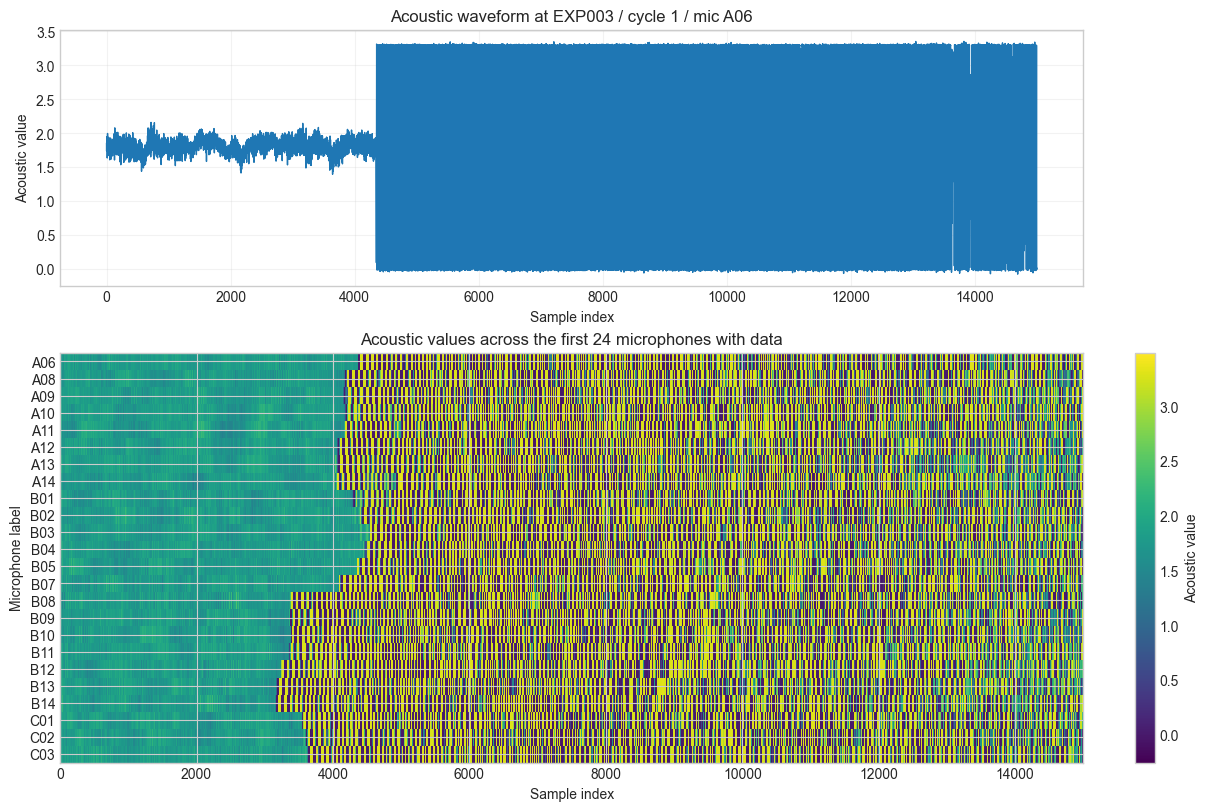
\includegraphics[width=0.5\textwidth]{figures/notebook-exports/rf_acoustic_position_waveform_heatmap.png}
    \caption{Acoustic waveform inspection for the position resolved by the joint \gls{rf}-acoustic notebook. The upper panel shows one microphone trace for \texttt{EXP003}/cycle~1, while the lower panel shows the corresponding waveform matrix for the first microphones with available data at the same acquisition cycle.}
    \label{fig:rf-acoustic-position-waveforms}
\end{figure}

\begin{figure}[t]
    \centering
    \begin{subfigure}[t]{0.48\textwidth}
        \centering
        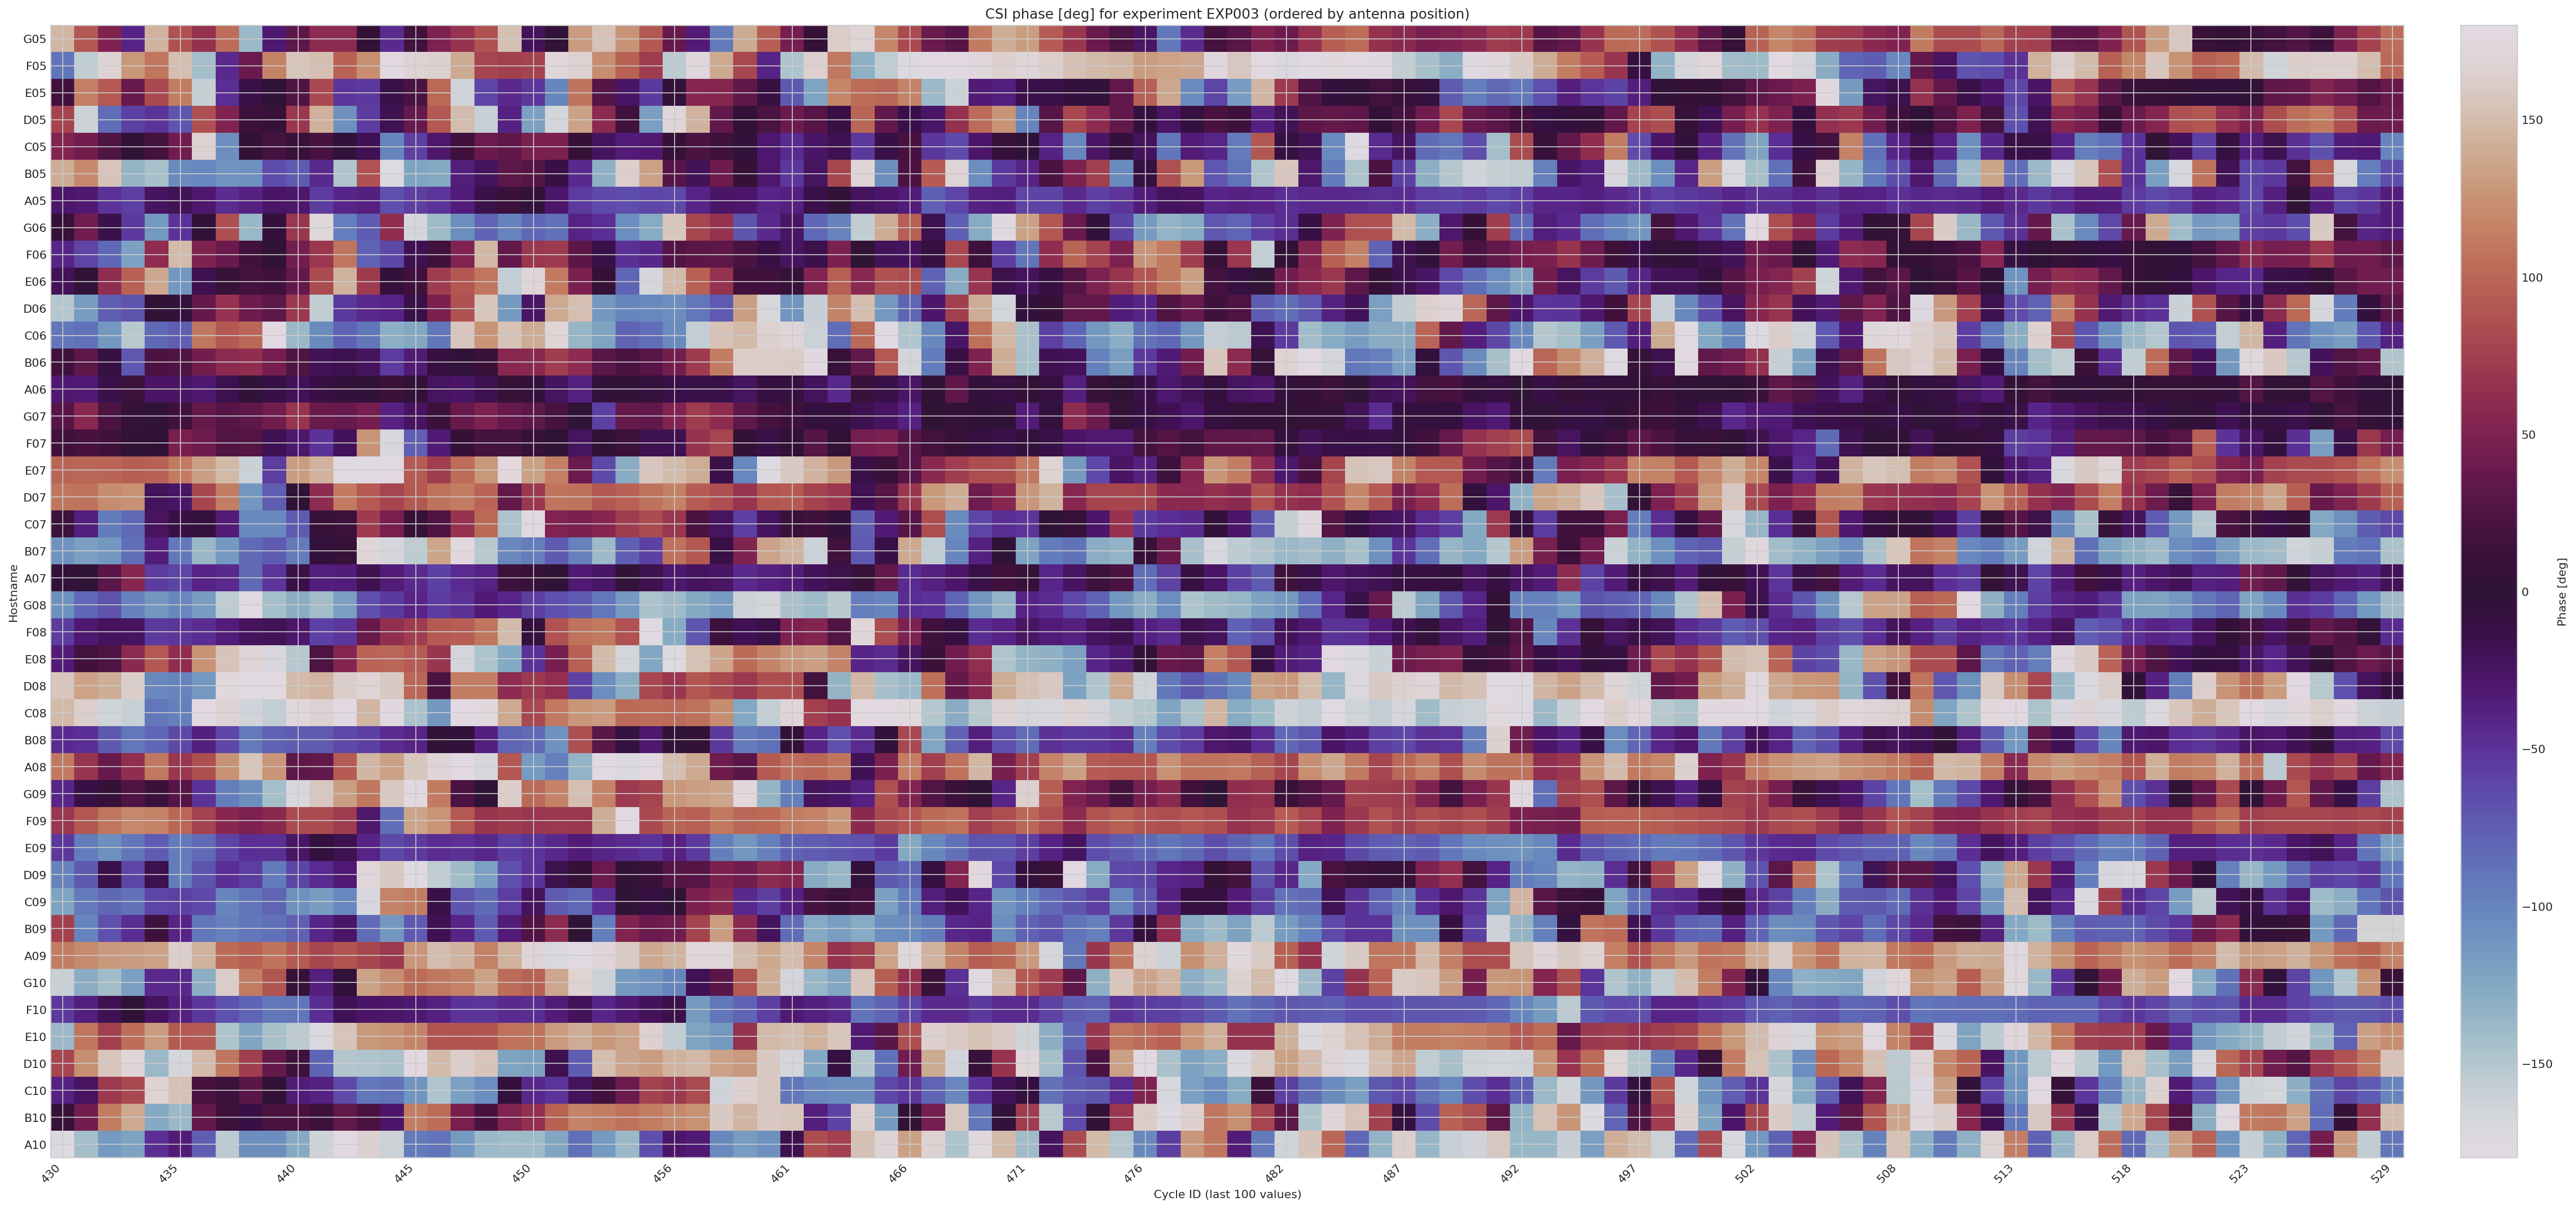
\includegraphics[width=\linewidth]{figures/notebook-exports/csi_position_phase_heatmap.png}
        \caption{\gls{csi} phase over the selected cycle window.}
    \end{subfigure}\hfill%
    \begin{subfigure}[t]{0.48\textwidth}
        \centering
        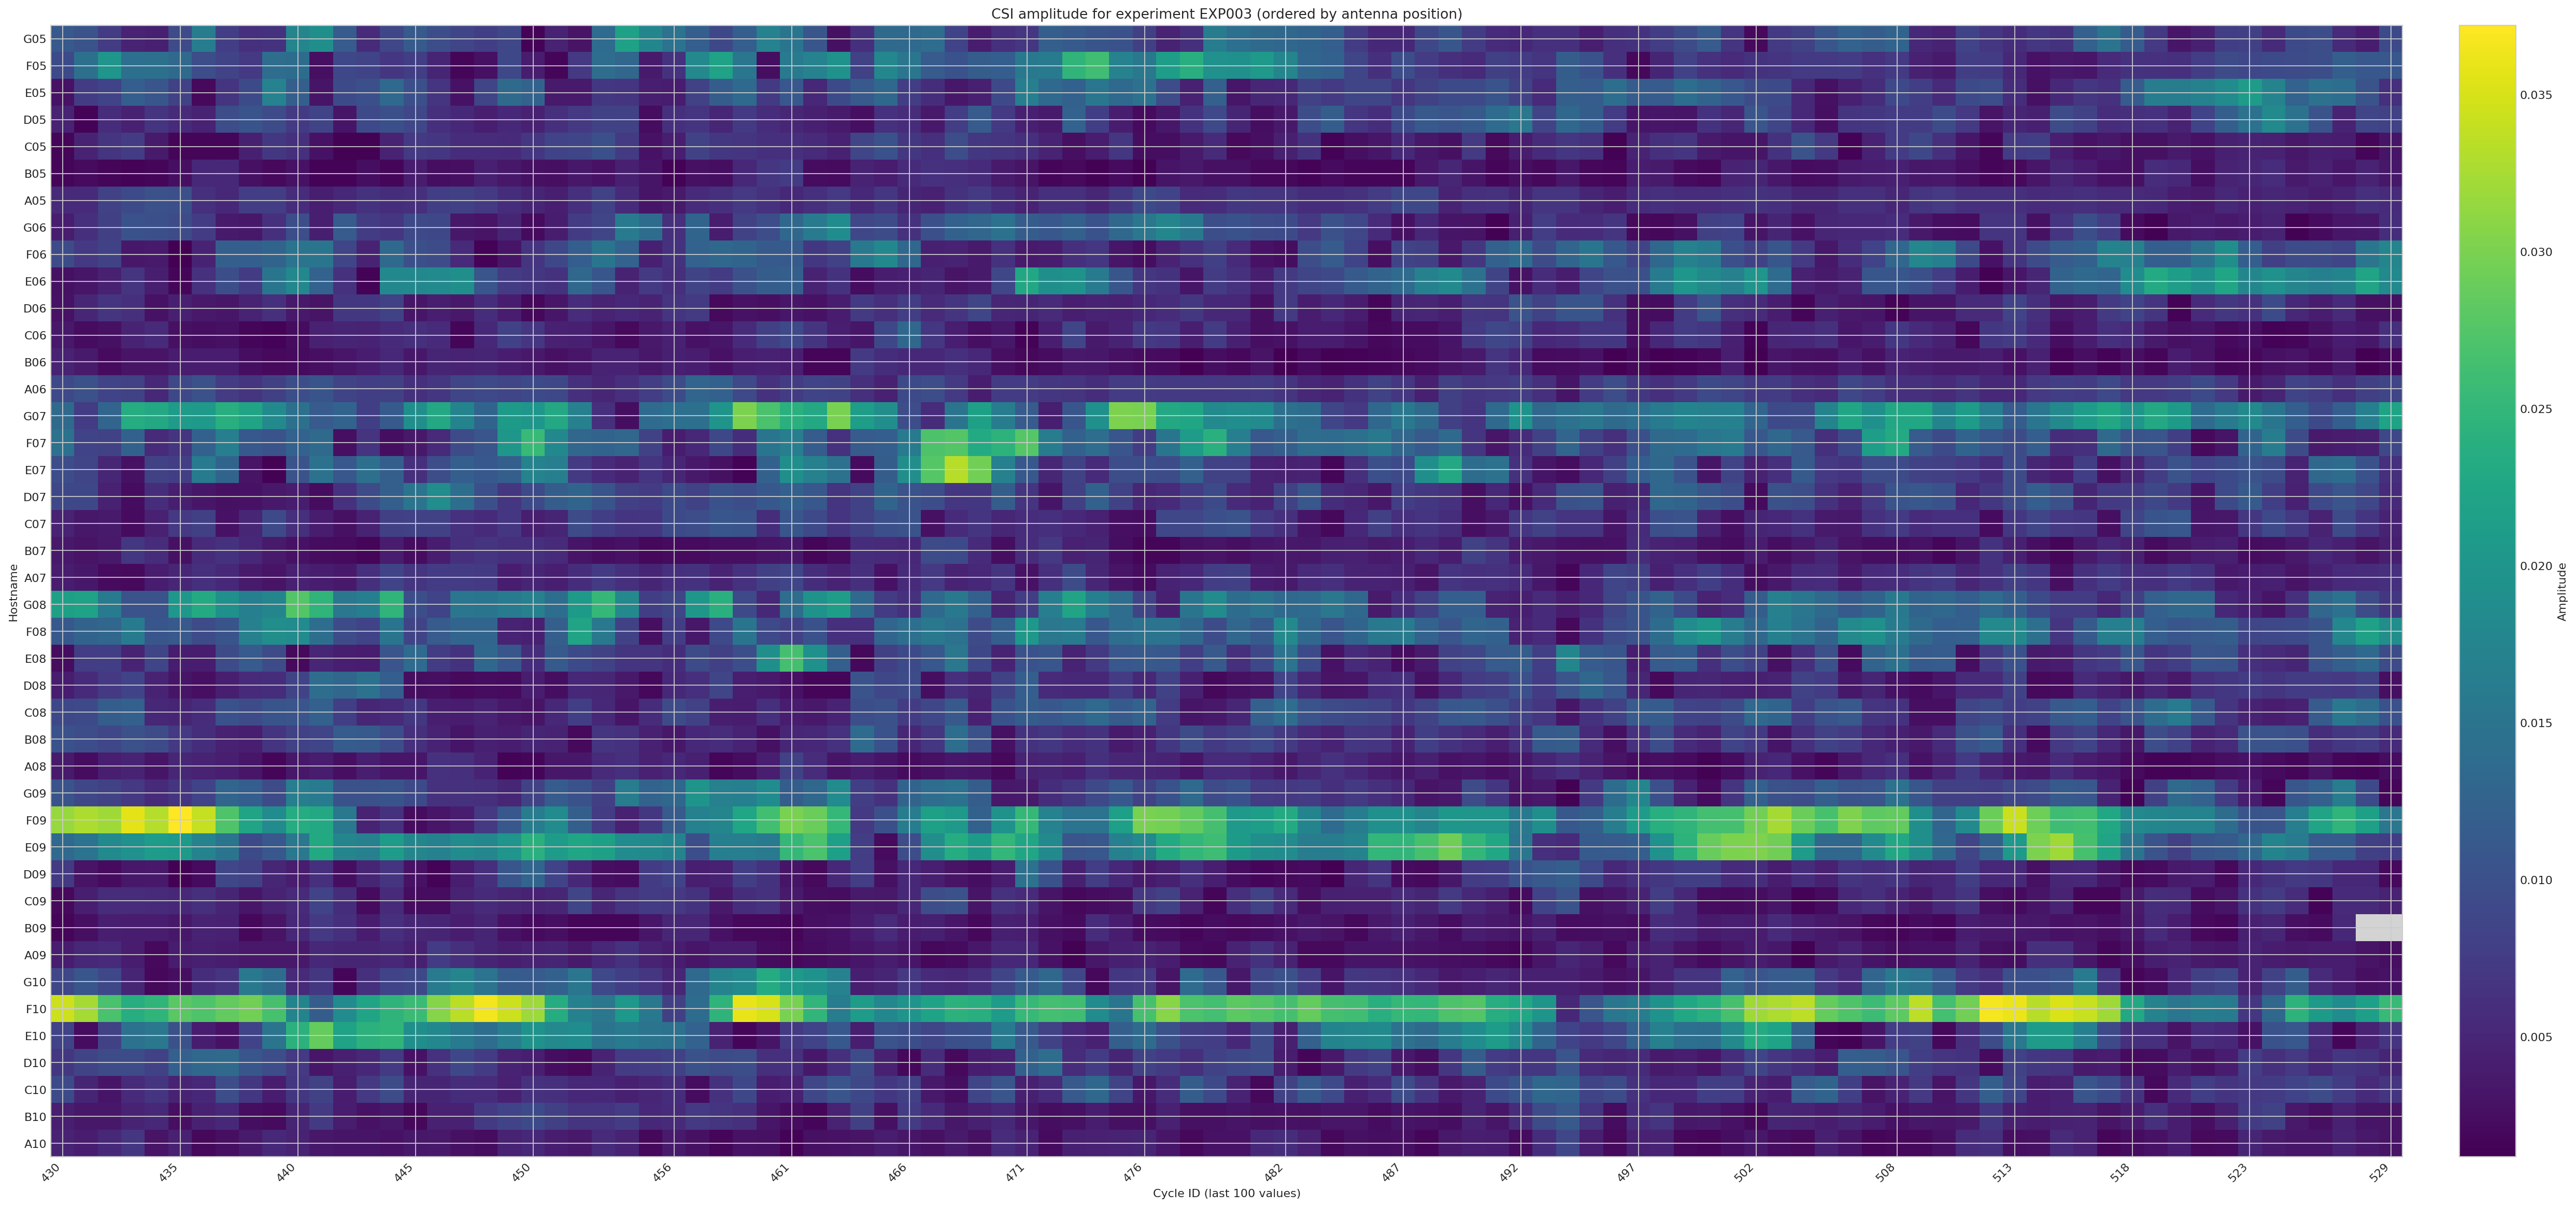
\includegraphics[width=\linewidth]{figures/notebook-exports/csi_position_amplitude_heatmap.png}
        \caption{\gls{csi} amplitude over the same cycle window.}
    \end{subfigure}
    \caption{Heatmaps from \texttt{tutorial\_csi\_per\_position.ipynb}. The rows are ordered ceiling receiver hostnames, and the columns show the final cycle IDs in the selected experiment window. Together they expose stable receiver-dependent structure and temporal variation in the \gls{rf} channel tensor.}
    \label{fig:csi-position-heatmaps}
\end{figure}


\begin{figure*}[b]
    \centering

\includegraphics[width=0.9\textwidth]{article/figures/correlation_graph_good_example.png}
    \caption{Ranging estimate example for cycle 304 EXP007 microphone C04 with the correlation values and LPF values. The correct peak resulting in the estimated range is determined using the peak-prominence algorithm. The estimated and ground-truth range is depicted.}
    \label{fig:correlation_graph_example}
\end{figure*}

\begin{figure}[]
    \centering
    
\includegraphics[width=\linewidth]{article/figures/paths.png}
    \caption{Four randomly generated walks. Red indicates a static point, and blue indicates points on the paths between static points.}
    \label{fig:generatedwalks}
\end{figure}

The post-processing workspace now makes the RF--acoustic positioning path concrete rather than merely hypothetical. It includes a graph-based walk generator and persisted train/test trajectory splits, with 2500 generated training walks and 50 held-out test walks. The test set positions are excluded from the training walks data.
The walk generator works by choosing a sequence of static flagged positions, and repeatedly performing Dijkstra's algorithm to find the shortest path from one static point to the next, along the rover measurement points. Static positions are introduced to perform acoustic positioning. The sequence of static points can either be randomly generated or manually specified. There is also an option to forbid the paths from containing specific points. Figure \ref{fig:generatedwalks} showcases four examples of randomly generated walks.

The acoustic positioning scripts operate on the static flagged positions in the paths by filtering the received signals, selecting anchor microphones, applying chirp pulse compression as depicted in Fig.~\ref{fig:correlation_graph_example}, estimating time-of-arrival ranges based on a peak-prominence algorithm, and by determining a least-squares position estimate for each rover stop. The most optimal peak-prominence-factor is determined for this dataset, resulting in a value equal to 0.24.  The current configuration uses up to 50 selected anchors per stop with sum-rate-based ranking due to the saturating operation mode of the microphones, which means that the released waveform data is already exercised by a full end-to-end model-based localization pipeline. 

The saved evaluation artifacts are strong enough to summarize as experimental evidence. The calibrated acoustic results cover 50 held-out paths and 550 localized rover stops. Across that set, the mean 2D positioning error is 0.110~m and the P90 value is equal to 0.195~m, while the mean 3D positioning error is 0.130~m and the P90 value is equal to 0.217~m. The accompanying ranging records contain 27500 anchor-wise distance estimates with mean absolute error 0.311~m. These values should be interpreted as documented baseline performance of the current model-based acoustic pipeline, not as an upper bound on what the dataset can support. At present, the \gls{rf} pipeline regarding positioning is still exploratory compared with the more complete acoustic ranging-and-localization path. \Cref{fig:capability-artifacts} illustrates tile-level interpretation of one synchronized \gls{rf} capture. This is a meaningful capability distinction for users who may be interested in fingerprinting, distributed channel modeling, RF-acoustic fusion, or direct positioning inference.

\begin{figure}[t]
    \centering
    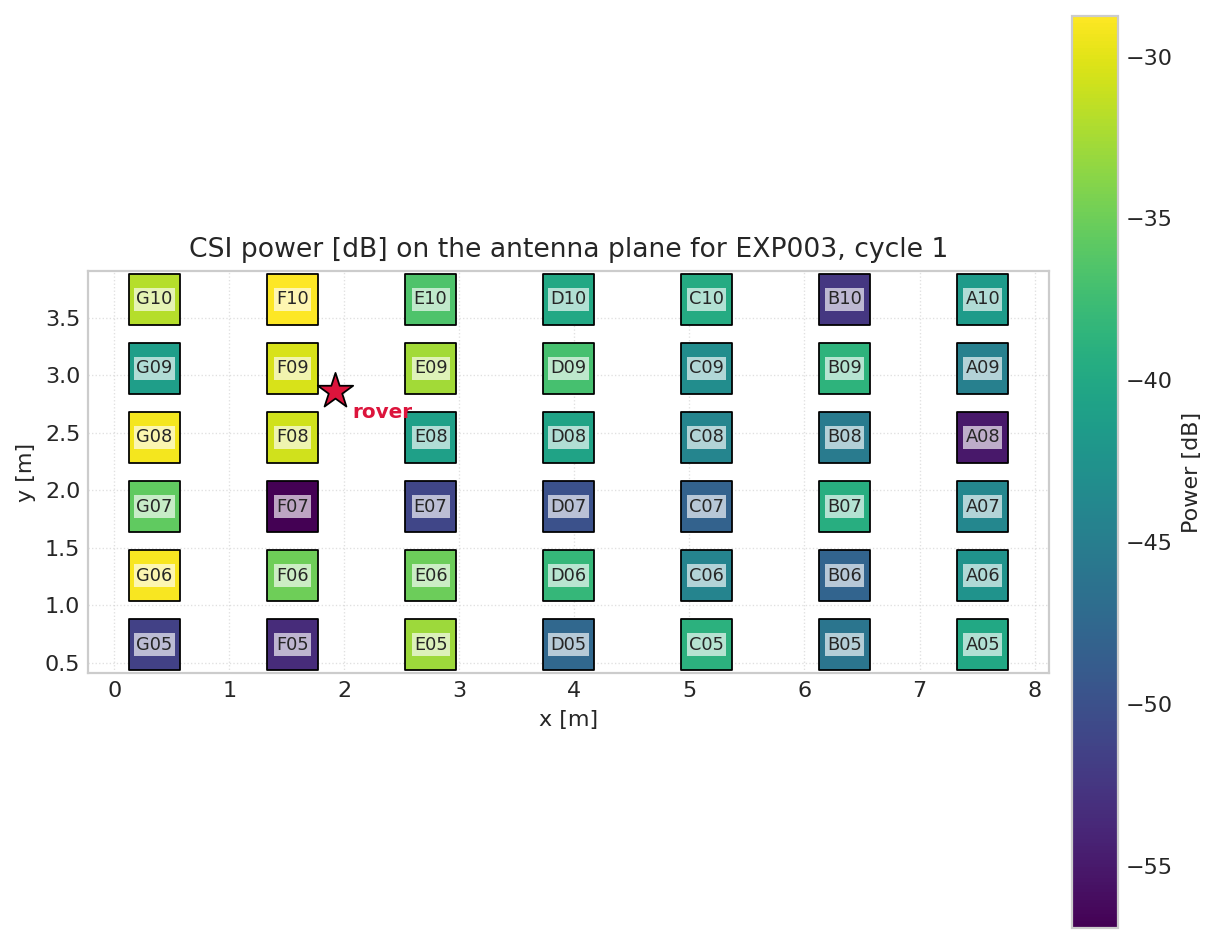
\includegraphics[width=\linewidth]{figures/notebook-exports/csi_spatial_power_snapshot.png}
    \caption{Example per-position \gls{rf} power snapshot over the 42 ceiling receivers.}\label{fig:capability-artifacts}
\end{figure}

The analysis workflow already demonstrates the most immediate downstream uses. The provided notebooks support:
\begin{itemize}
    \item campaign-level trajectory inspection and measurement-cloud visualization;
    \item overview heatmaps of \gls{csi} phase and amplitude over the measurement set;
    \item single-position spatial snapshots across the 42 ceiling receivers;
    \item joint \gls{rf}-acoustic inspection at a selected rover stop;
    \item export of movie sequences showing spatial evolution of phase and power.
\end{itemize}
Taken together with the acoustic and \gls{rf} post-processing scripts, these are not promised future tasks, they are concrete analyses already represented by scripts, notebooks, and exported figures in the present project release.





\section{Discussion and Interpretation Caveats}
\label{sec:discussion}

The ARFT dataset's main strength is not just its multi-modal measurements, but its explicit distinction between the logged campaign and the analysis-ready subset. As a result, transparency about the currently merged 9 (rather than 12) experiments is essential. The completeness report should therefore be read on two levels: rover logs show what was physically traversed, while the merged \gls{rf}-acoustic dataset shows what is available for channel analysis. This is why EXP001, EXP002, and EXP004 remain relevant to the campaign narrative, despite not contributing processed \gls{rf} and acoustic data to the current merged set.

The second caveat is structural. The \texttt{cycle\_id} axis in the merged \gls{rf} NetCDF is a shared union axis across experiments, not a guarantee that every experiment occupies every cycle index. Validity is encoded by the availability masks, not merely by coordinate presence. Any downstream study that ignores \texttt{csi\_available} or \texttt{position\_available} risks accidentally treating absent data as zero-valued data or assuming that coordinate existence implies measurement existence.

Furthermore, the measurements were performed statically. Therefore, especially the slow-propagating and long reverberating acoustic waves should be handled as static measurements to perform realistic positioning.

\section{Conclusion}

This paper presents ARFT as a synchronized measurement campaign and data release rather than a benchmark. It integrates rover motion with Qualisys positioning, acoustic sensing, and distributed ceiling-tile \gls{rf} measurements in Techtile. The current release comprises 12 experiments (6735 rover stops), including a merged 9-experiment \gls{rf} dataset (5011 cycles, 210068 \gls{csi} values), 5855 acoustic cycles, and a fully aligned tri-modal subset of 5011 cycle pairs.

The key contribution is clarity: ARFT supports spatial analysis, tile-level \gls{rf} inspection, multimodal cycle alignment, and baseline acoustic localization, provided the appropriate completeness subset is used. By explicitly documenting coverage, processing, example scripts and limitations, this work establishes a reliable dataset for distributed communication and multimodal sensing research~\faicon{github}\footnote{\url{https://github.com/techtile-by-dramco/ELLIIIT-dataset-26/}}.


\section*{Acknowledgment}
This work was supported by the IoF fund of KU Leuven allocated to the `POMPOEN' project. Furthermore, a special thanks to the ELLIIT community to support us and to provide the impetus to create this dataset. Thank you to Geoffrey Ottoy and Bert Cox for the collaboration with the realization of the Techtile infrastructure.


\printbibliography%

\end{document}
